\documentclass{article}
%
% Demo of the mcode package from 
% http://www.mathworks.co.uk/matlabcentral/fileexchange/8015-m-code-latex-package
% Updated 06 Mar 2014
%

\usepackage{graphicx}
\usepackage{wrapfig}
\usepackage{mathtools}
\usepackage{mathrsfs}
\usepackage{enumitem}
\usepackage{pdflscape}
\graphicspath{ {images/} }

\usepackage{float}
% load package with ``framed'' and ``numbered'' option.
\usepackage[framed,numbered,autolinebreaks,useliterate]{mcode}

% something NOT relevant to the usage of the package.
\usepackage{url}
\setlength{\parindent}{0pt}
\setlength{\parskip}{18pt}


% //////////////////////////////////////////////////

\begin{document}

\title{Homework 9 - Optimal Control Systems}
\author{Erivelton Gualter dos Santos, 2703806}
\date{}

\maketitle 

\section{Steepest Descent Solution}

The following figures (1, 2 and 3) are the results for the steepest descent method for the initial states $[0.5 \:\: 0]^T$, Initail control equal $1$ and step size $\tau$ equal to $0.25$. It reach the optimal trajectory in 48 interactions. 

\begin{figure}[H]
\centering
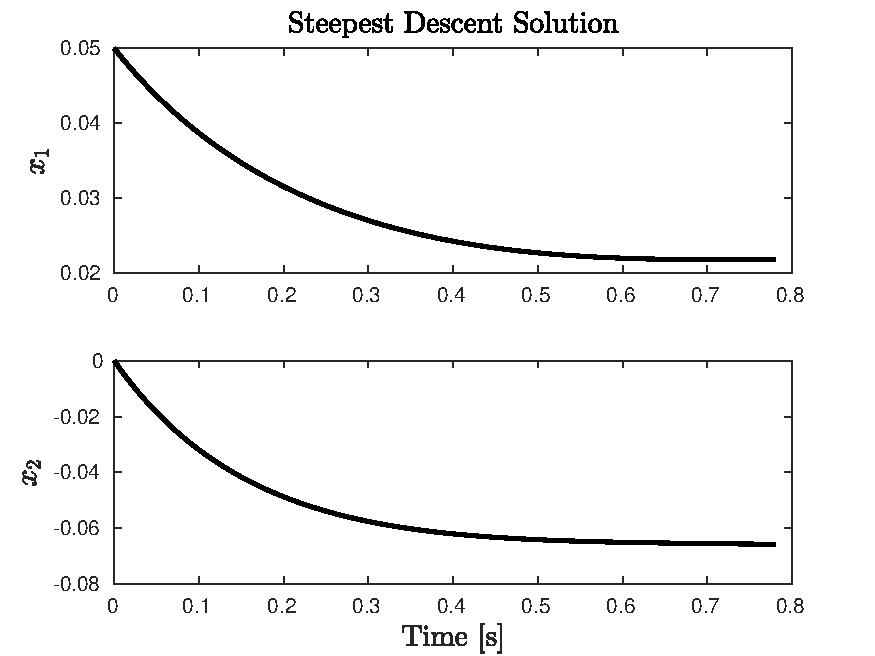
\includegraphics [width=3.5in]{fig1}
\caption{Optimal Control Trajectory}
\end{figure}

\begin{figure}[H]
\centering
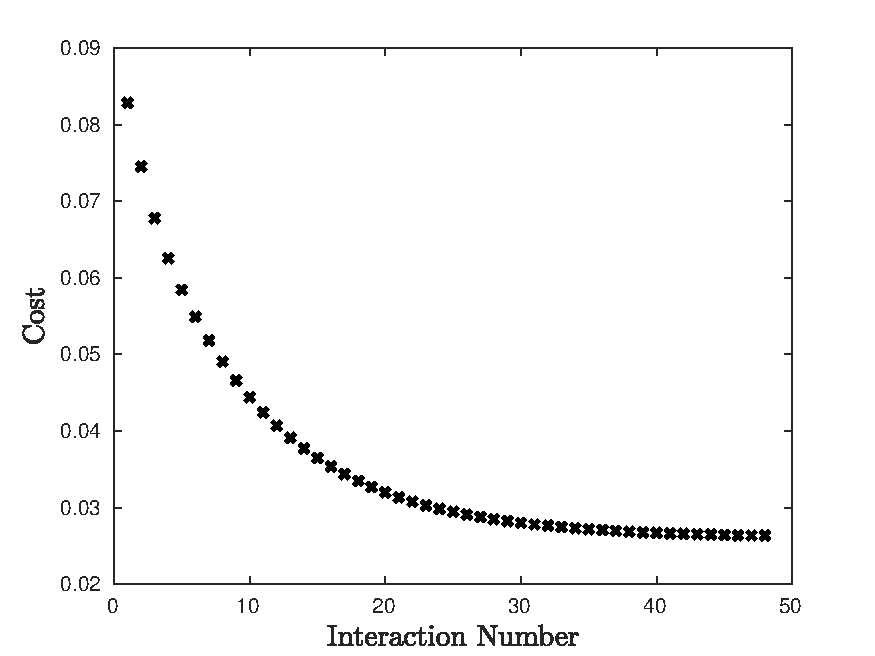
\includegraphics [width=3.5in]{fig2}
\caption{Performance Measure as a function of number of interactions}
\end{figure}

\begin{figure}[H]
\centering
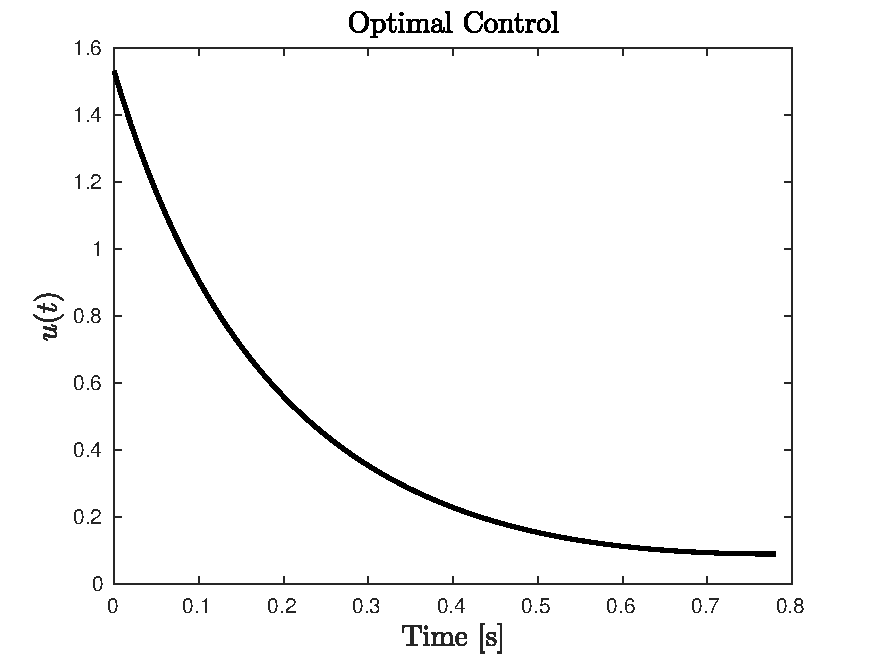
\includegraphics [width=3.5in]{fig3}
\caption{Optimal Control}
\end{figure}

\begin{table}[H]
\centering
\caption{Number of interaction for different initial conditions}
\label{my-label}
\begin{tabular}{cccr} \hline
Initial Control & Initial eps & Number of iterations required & \multicolumn{1}{c}{Minimum value of J} \\ \hline
1               & 0.25        & 48                            & 0.026260622628662                      \\
1               & 0.5         & 25                            & 0.026260622628662                      \\
0               & 0.25        & 19                            & 0.026341012128041                      \\
0               & 0.1         & 42                            & 0.026347117309669                      \\
0               & 0.01        & 386                           & 0.026353420232887        \\
\hline             
\end{tabular}
\end{table}

From the table 1, it is clear that the initial condition makes a substantial difference relating to the number of interactions. Also, the magnitude of the gradient descent step size says how fast it will perform the new operation.

\section{Variation of Extremal Solution}

The following figures (4, 5 and 6) are the results for the Variation of Extremal method for the initial states $[0.5 \:\: 0]^T$ and $P0 = [1 \: 0.5]^T$. It reach the optimal trajectory in 5 interactions. 

\begin{figure}[H]
\centering
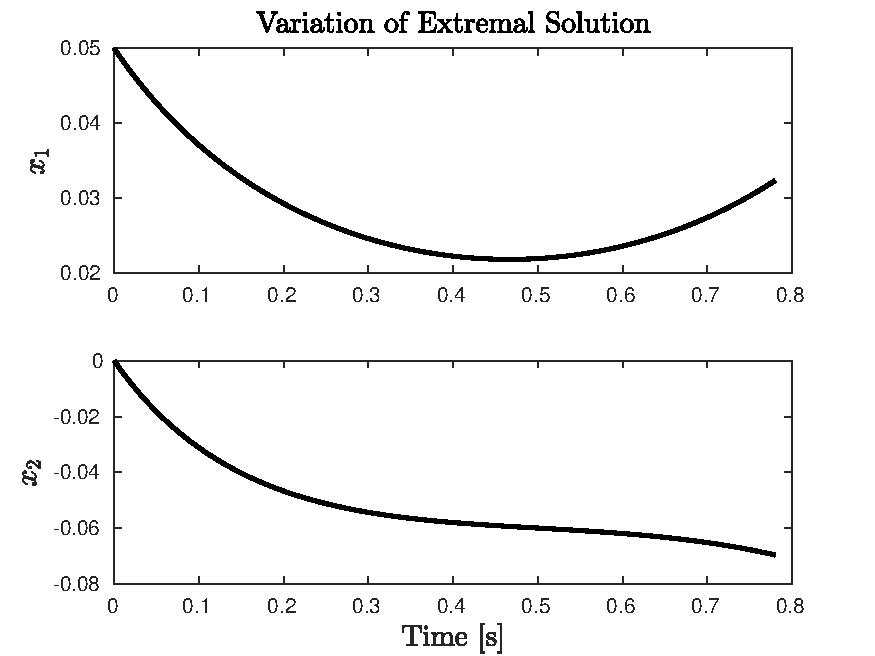
\includegraphics [width=3.5in]{fig4}
\caption{Optimal Control Trajectory}
\end{figure}

\begin{figure}[H]
\centering
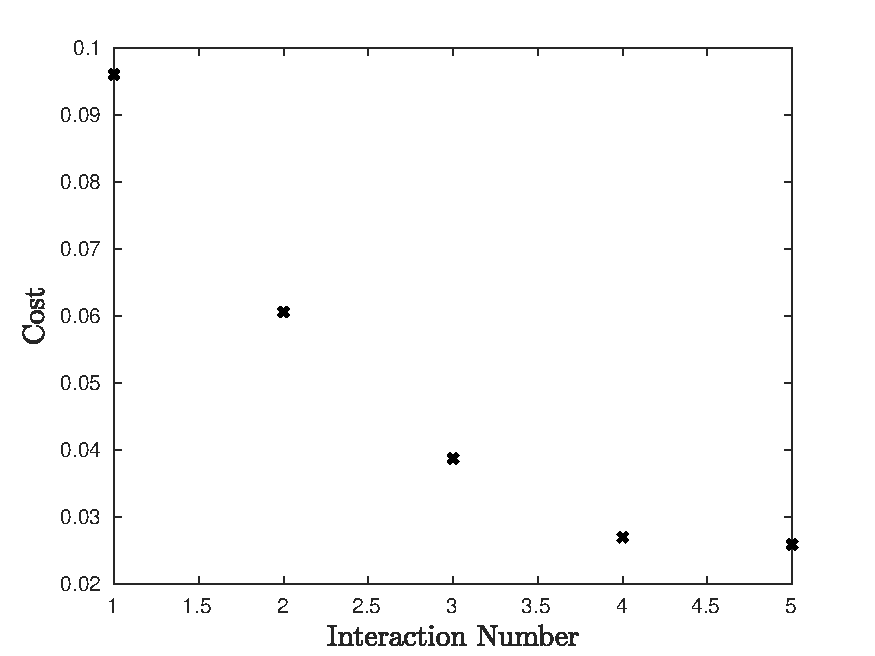
\includegraphics [width=3.5in]{fig5}
\caption{Performance Measure as a function of number of interactions}
\end{figure}

\begin{figure}[H]
\centering
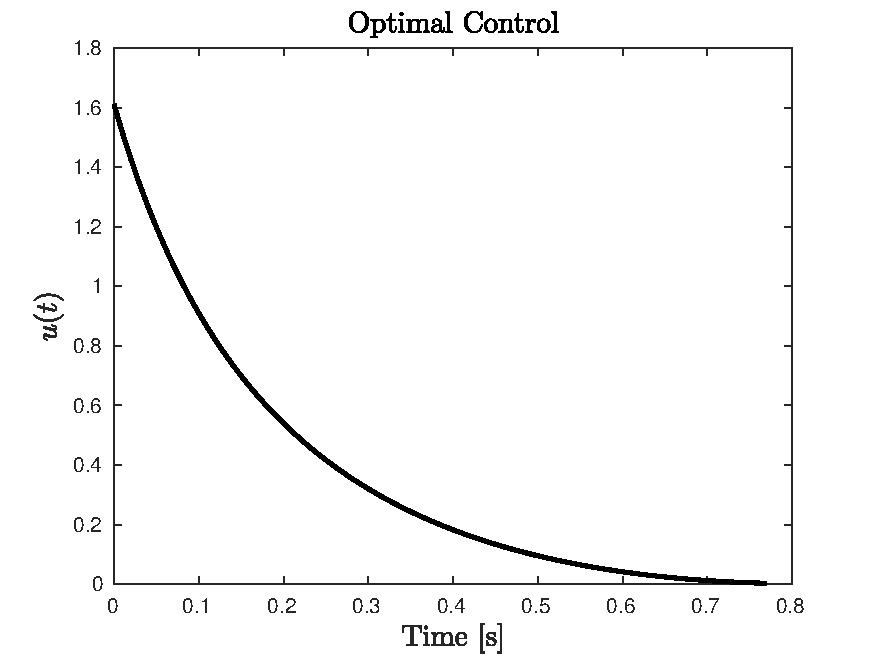
\includegraphics [width=3.5in]{fig6}
\caption{Optimal Control}
\end{figure}

\begin{table}[H]
\centering
\caption{Number of interaction for different initial conditions}
\label{my-label}
\begin{tabular}{cccr} \hline
P\_1(0) & P\_2(0) & Number of iterations required & \multicolumn{1}{c}{Minimum value of J} \\ \hline
1       & 0.5     & 5                             & 0.025950108657380                      \\
2       & 1       & 33                            & 0.025934192378058                      \\
2       & 2       & 37                            & 0.025932988188449                     \\
\hline
\end{tabular}
\end{table}

Depending of the initial conditions, the simulation can reach the optimal solution really fast, or can take several hundreds interactions. Therefore, it must be choose carefully and based in the system.

 
\begin{lstlisting}
% Book: Optimal Control Theory: An introduxtion by Donald E. Kirk
%
% Erivelton Gualter, 03/26/2018
% Problem 6.34

clc;
clear all; 
close all;

% Simulation Parameters
tf = 0.78;
dt = 0.01; % time step
t = 0 : dt : tf;
N = length(t); % number of time steps
X0  = [0.05; 0];      

% Parameters
R = 0.1;
eps = 0.25;

u = ones(size(t));

NormHu = inf;
JArr = [];

for iter = 1 : Inf
    % Simulatio system
    X = X0;
    for k=1 : length(t)-1
        x1 = X(1,k);
        x2 = X(2,k);

        xd1 = -2*(x1+0.25) + (x2+0.5)*exp(25*x1/(x1+2)) -(x1+0.25)*u(k);
        xd2 = 0.5 - x2 - (x2+0.5)*exp(25*x1/(x1+2));

        XDOT = [xd1; xd2];

        X(:,k+1) = X(:,k) + XDOT*dt;
    end

    % Compute the costate
    p = zeros(2, N); 
    p(1, N) = 0;
    p(2, N) = 0;
    
    for i = N-1 : -1 : 1
        x1 = X(1,i+1);
        x2 = X(2,i+1);
        p1 = p(1,i+1);
        p2 = p(2,i+1);

        pDot(1, i) = -2*x1 + 2*p1 - ...
                  p1*(x2+0.5)*(50/(x1+2)^2)*exp(25*x1/(x1+2)) + ...
                  p1*u(i+1) + p2*(x2+0.5)*(50/(x1+2)^2)*exp(25*x1/(x1+2));
        pDot(2, i) = -2*x2 - p1*exp(25*x1/(x1+2)) + p2*(1 + exp(25*x1/(x1+2)));

        p(:, i) = p(:, i+1) - dt * pDot(:, i);
    end

    % Compute cost
    J = dt*trapz(X(1,:).^2 + X(2,:).^2 + R*u.^2);
    JArr = [JArr J];
       
    % Compute the partial of the Hamiltonian with respect to the control
    for i=1:N
        Hu(i) = 2*R*u(i)-p(1,i)*(X(1,i)+0.25);
    end
    
    NormHu = sqrt(dt * trapz(Hu.^2));
    disp(['Iteration # ',num2str(iter),', Hu = ',num2str(NormHu)]);
    Optmail
    if NormHu < 0.01
        break;
    end
    u = u - eps * Hu;
end

%%
close all
f1 = figure;
subplot(211); plot(t, X(1,:), '-k','LineWidth',2)
    title('Steepest Descent Solution', 'Interpreter','Latex', 'FontSize',14);
    ylabel('$x_1$', 'Interpreter','Latex', 'FontSize',14);
subplot(212); plot(t, X(2,:),'-k','LineWidth',2)
    ylabel('$x_2$', 'Interpreter','Latex', 'FontSize',14);
    xlabel('Time [s]', 'Interpreter','Latex', 'FontSize',14);

f2 = figure;
plot(JArr,'xk','LineWidth',2);
    ylabel('Cost', 'Interpreter','Latex', 'FontSize',14);
    xlabel('Interaction Number', 'Interpreter','Latex', 'FontSize',14);

f3 = figure;
plot(t,u, '-k','LineWidth',2);
    title('Optimal Control', 'Interpreter','Latex', 'FontSize',14);
    ylabel('$u(t)$', 'Interpreter','Latex', 'FontSize',14);
    xlabel('Time [s]', 'Interpreter','Latex', 'FontSize',14);
    
saveFigureToPdf('fig1',f1);
saveFigureToPdf('fig2',f2);
saveFigureToPdf('fig3',f3);

% Book: Optimal Control Theory: An introduxtion by Donald E. Kirk
%
% Erivelton Gualter, 03/26/2018
% Problem 6,34 and 6.35

clc;
clear all; 
close all;

% Simulation Parameters
tf = 0.78;
dt = 0.01; % time step
t = 0 : dt : tf;
N = length(t); % number of time steps

% Parameters
R = 0.1;

P0 = [1; 0.5];
% P0=[1.0782; 0.1918];
X0  = [0.05; 0];

JArr = [];

for iter = 1 : Inf

    % Simulatio system
    X = X0;
    P = P0;
    for k=1 : N-1
        x1 = X(1,k);
        x2 = X(2,k);
        p1 = P(1,k);
        p2 = P(2,k);

        u(k) = p1*(x1+0.25)/(2*R);
        
        xd1 = -2*(x1+0.25) + (x2+0.5)*exp(25*x1/(x1+2)) -(x1+0.25)*u(k);
        xd2 = 0.5 - x2 - (x2+0.5)*exp(25*x1/(x1+2));        
        pd1 = -2*x1 + 2*p1 - ...
                  p1*(x2+0.5)*(50/(x1+2)^2)*exp(25*x1/(x1+2)) + ...
                  p1*u(k) + p2*(x2+0.5)*(50/(x1+2)^2)*exp(25*x1/(x1+2));
        pd2 = -2*x2 - p1*exp(25*x1/(x1+2)) + p2*(1 + exp(25*x1/(x1+2)));
        
        XDOT = [xd1; xd2];
        PDOT = [pd1; pd2]; 

        X(:,k+1) = X(:,k) + XDOT*dt;
        P(:,k+1) = P(:,k) + PDOT*dt;
    end

    J = dt*trapz(X(1,1:end-1).^2 + X(2,1:end-1).^2 + R*u.^2);    
    JArr = [JArr J];

    p = P(:,end);
    ErrorNorm = norm(p);
    if ErrorNorm < 0.01
        break
    end
    if (norm(P(1,end)) + norm(P(2,end))) < 1e-5
        break;
    end
    disp(['Cost = ', num2str(J), ', Error norm = ', num2str(ErrorNorm)]);

    
    % integrate the Px and Pp matrices
    Px = zeros(2,2);
    Pp = eye(2);
        
    for i = 1 : N
        x1 = X(1,i);
        x2 = X(2,i);
        
        alpha = exp(25*x1/(x1+2));
        d2Hdpdx = [-2+50*(x2+0.5)*alpha/(x1+2)^2-(x1+0.25)*p1/R, alpha; ...
              -50*(x2+0.5)*alpha/(x1+2)^2, -1-alpha];
        d2Hdp2 = [-(x1+0.25)^2/(2*R), 0; 0, 0];
        d2Hdx2 = [-2+(p2-p1)*(100*(23-x1)*(x2+0.5)/(x1+2)^4)*alpha + p1^2/(2*R), 50*(p2-p1)*alpha/(x1+2)^2; ...
                50*(p2-p1)*alpha/(x1+2)^2,  -2];
        d2Hdxdp = d2Hdpdx';
    
        Pxdot = d2Hdpdx * Px + d2Hdp2 * Pp;
        Ppdot = d2Hdx2 * Px - d2Hdxdp * Pp;
        Px = Px + Pxdot * dt;
        Pp = Pp + Ppdot * dt;
    end
    P0 = P0 - inv(Pp) * p % updated p(0) guess
end

%%
close all
f4 = figure;
subplot(211); plot(t, X(1,:), '-k','LineWidth',2)
    title('Variation of Extremal Solution', 'Interpreter','Latex', 'FontSize',14);
    ylabel('$x_1$', 'Interpreter','Latex', 'FontSize',14);
subplot(212); plot(t, X(2,:),'-k','LineWidth',2)
    ylabel('$x_2$', 'Interpreter','Latex', 'FontSize',14);
    xlabel('Time [s]', 'Interpreter','Latex', 'FontSize',14);

f5 = figure;
plot(JArr,'xk','LineWidth',2);
    ylabel('Cost', 'Interpreter','Latex', 'FontSize',14);
    xlabel('Interaction Number', 'Interpreter','Latex', 'FontSize',14);

f6 = figure;
plot(t(1:end-1),u, '-k','LineWidth',2);
    title('Optimal Control', 'Interpreter','Latex', 'FontSize',14);
    ylabel('$u(t)$', 'Interpreter','Latex', 'FontSize',14);
    xlabel('Time [s]', 'Interpreter','Latex', 'FontSize',14);
    
saveFigureToPdf('fig4',f4);
saveFigureToPdf('fig5',f5);
saveFigureToPdf('fig6',f6);
\end{lstlisting}

You can access the code at: https://github.com/EriveltonGualter/EEC-744-Optimal-Control-Systems



\end{document}
